\section{Introduction}
\label{sec:intro}

%SSO的特点
%SSO的现状
Single sign-on (SSO) systems, such as OAuth~\cite{rfc6749}, OpenID Connect~\cite{OpenIDConnect} and SAML~\cite{SAML}, have been widely adopted nowadays as a convenient web authentication mechanism. SSO delegates user authentication from websites, so-called relying parties (RPs), to a third party, so-called identity providers (IdPs), so that users can access different services at cooperating sites via a single authentication attempt. Using SSO, a user no longer needs to maintain multiple credentials for different RPs, instead, she maintains only the credential for the IdP, who in turn will generate corresponding \emph{identity proofs} for those RPs. Moreover, SSO shifts the burden of user authentication from RPs to IdPs and reduces security risks and costs at RPs. As a result, SSO has been widely integrated with modern web systems.
Our study shows that 80\% of the Alexa top-100 websites~\cite{Alexa} support SSO services and study on the Alexa top 1 million websites has found that 6.30\% of websites support  SSO~\cite{GhasemisharifRC18}.
Meanwhile, many email and social networking providers such as Google, Facebook, Twitter, etc. have been actively serving as social identity providers to support social login.


%SSO系统的安全问题,需要保护identity proof的完整性,机密性,绑定性
%完整性:使用公开的为受保护的信息作为identity proof
%机密性:保证由IdP发送给对应的RP,并且传输过程中通道、user agent都是受到保护的
%绑定性:identity proof一定要与对应的RP实现绑定
A fundamental requirement of SSO systems is secure authentication~\cite{SPRESSO}, which should ensure that it is impossible (1) for an adversary to log in to an honest RP as an honest user (i.e., impersonation); and (2) for an honest user to log in to an honest RP as someone else such as an adversary (i.e., identity injection).
Extensive study have been performed on existing SSO systems exposing various vulnerabilities~\cite{ChenPCTKT14, FettKS16,WangCW12,ZhouE14,WangZLG16,YangLLZH16,SomorovskyMSKJ12,MohsenS16}. It is commonly recognized that SSO security highly depends on secure generation and transmission of identity proofs: (1) the identity proof should be generated in a way that it can never be forged or tampered. For example, when Google used user's attributes with a signature as the identity proof~\cite{WangCW12}, {\color{red}the adversary is able to bypass the verification of part of attributes in the identity proof. The root cause is that RP relies on the IdP signed user's attributes to identify the user, however, when the adversary acts as the user, it is able to modify the request and repose between RP and IdP transmitted by user, which allows the adversary add any honest user's attributes in the IdP's response and RP would accept all of them without verifying the signature. Finally the adversary is able to log in to the RP as the honest user}.
(2) The identity proof should be generated in a way that it is bound to the requesting RP. For example, if an identity proof is generated with nonbinding data such as access tokens in OAuth 2.0, an adversary such as a malicious RP is able to log in to an honest RP as the honest user~\cite{ChenPCTKT14, WangZLG16}.
%the parts of IdP developer choose the data (e.g., access token in OAuth 2.0) unbound with specific RP as the identity proof, which results in that the malicious RP is able to collect user's identity proof and use it to log in to other RPs.
(3) The identity proof should only be obtained by the requesting RP. For example, in some mobile SSO implementations using WebView~\cite{MohsenS16}, as the url check is not supported which the malicious RP app invokes the IdP's web site in its Webview, the adversary is able to steal the identify proof of an honest user when the app cheats her to consider it as another honest RP.

%第二段:
%SSO 引入新的隐私问题
%IdP知道用户登录哪个RP
%RP之间可以合谋知道同一个用户登录哪些RP
The wide adoption of SSO also raises new privacy concerns regarding online user tracking and profiling~\cite{maler2008venn,NIST2017draft}. In a typical SSO authentication session, for example the OpenID Connect (OIDC) authentication flow as shown in Fig.~\ref{fig:OpenID}, when a user attempts to log in to an RP, the authentication request is redirected from the RP to the IdP, which generates an identify proof containing information about the user (e.g., user identifier and other authorized user attributes) and the requesting RP (e.g., RP identifier, URL, etc.). If a common user identifier is issued by the IdP for a same user across different RPs or a user's identifiers can be derived from each other, which is the case even in several widely deployed SSO systems~\cite{BrowserID,SPRESSO}, collusive RPs could not only track her online traces but also correlate her attributes across the sites~\cite{maler2008venn}. We refer to this as {\em RP-based identity linkage}. Moreover, when a user leverages the identity issued by one IdP across multiple RPs, the IdP acquires a central role in web authentication, which enables it to collect information about the user's logins at different sites~\cite{maler2008venn}. Since the information of the RP is necessary in the construction of identity proof to make sure it is bound with specific RP~\cite{ChenPCTKT14, WangZLG16}, any interested IdP can easily discover all the RPs accessed by a user and reconstruct her access traces by the unique user identifier. We refer to this as {\em IdP-based access tracing}. Both RP-based identity linkage and IdP-based access tracing could lead to more severe privacy violations.




%第三段:
%google and facebook的负面新闻
%1. service provider(如DNS)知道你访问了,可以带来很多问题。但是还是不同的,DNS里profile需要评估的是two behavior vectors的similarities,而IdP中都不需要,因为IdP能够区分two behavior vectors 是否来自相同节点。

Meanwhile, large IdPs, especially social IdPs like Google and Facebook, are known to be interested in collecting users' online behavioral information for various purposes (e.g., Screenwise Meter~\cite{googlenews}, Onavo~\cite{Onavo}). By simply serving the IdP role, these companies can easily collect a large amount of continuous data to reconstruct users' online traces. %Unlike other privacy risks, such as user session re-identification that requires to compute the similarity between users' DNS queries~\cite{DNS},
Moreover, many service providers are also hosting a variety of web services, which make them easy to link the same user's multiple logins in each RP as the unique user identifier is contained in the identity proof. Through internal integration, they could obtain rich information from SSO data to profile their clients.



While the privacy problems in SSO have been widely recognized~\cite{maler2008venn,NIST2017draft}, only a few solutions have been proposed to protect user privacy~\cite{persona,SPRESSO}. Among them, Pairwise Pseudonymous Identifier (PPID)~\cite{OpenIDConnect, SAMLIdentifier} is a most straightforward and commonly accepted solution to defend against RP-based identity linkage, which requires the IdP to create different user identifiers for the user when she logs in to different RPs. In this way, even multiple malicious RPs collude with each other across the system, they cannot link the  pairwise pseudonymous identifiers of the user and track which RPs she has visited. As a recommended practice by NIST~\cite{NIST2017draft}, PPID has been specified in many widely adopted SSO standards including OIDC~\cite{OpenIDConnect} and SAML~\cite{SAMLIdentifier}.

However, PPID-based approaches cannot prevent the IdPs from tracking at which RPs users log in, since pseudonymous identifiers are generated by IdP which only hide users' identity from the RPs. To authenticate a user, the IdP has to know her identity. To the best of our knowledge, there are only two approaches (i.e., BrowserID~\cite{BrowserID} and SPRESSO~\cite{SPRESSO}) being proposed so far to prevent IdP-based access tracing. Both adopt the idea of hiding RPs' identities from the IdP during the construction and transmission of identity proofs. In particular, the identity proof in BrowserID (and its prototype system known as Mozilla Persona~\cite{persona} and Firefox Accounts~\cite{FirefoxAccount}) is combined with two parts, the binding of the public key generated by the user with her email (as the user identifier) signed by IdP as the user certificate (UC) and the origin of the RP signed by user's private key as the identity assertion (IA). The core idea of BrowserID is that the IdP-generating part of identity proof does not contains any RP's identity and the work of binding identity proof with RP is shift to the user. 
% uses email address as user identifier, and lets the IdP bind the public key generated by the user with her email. The identity proof , the signed with the corresponding private key of the user and transmitted to the RP via the user. 
With the user as the proxy, the IdP does not know RPs' identities throughout the authentication process. 
In SPRESSO, the RP generates a dynamic pseudonymous identifier by encrypting its domain and a nonce, and passes it to the IdP through the user to create the identity proof, which is returned to the RP through a trusted third party, called forwarder, chosen by the RP itself. While forward transmitting the identity proof, it decrypts the encrypted RP domain to make sure the identity proof only sent to the requesting RP, however, the identity proof is encrypted by another RP generated symmetric key before transmitting to avoid the forward knowing the user's identity from identity proof, which will result in the forward tracing the user. As it designed in SPRESSO, the user email is adopted as the user identifier for identity proof generating. 

%In BrowserID, the identity proof is signed with the private key generated by user, and transmitted to the RP through the user directly,  while the corresponding  public key is bound with users' email by IdP who need not obtain the information of accessed RP. In SPRESSO, RP encrypts its domain and a nonce as the identifier, so that the real identity of RP is never exposed to IdP, while the identity proof is transmitted to the RP through a trusted entity (named FWD) who doesn't know the user's identity.




%用户和每一个RP分别在IdP处有长期不变的ID,分别称为ID_U和ID_RP;IdP为用户签发的identity proof中存在着连接ID_U和ID_RP的ID,称为ID_U^Proof;用户在每一个RP处都有长期不变的Account。
%在每一次identity proof产生的过程中(也就是每一次log in rp),IdP会产生绑定了ID_U和ID_RP的identity proof
%原始的SSO方案中,会同时暴露ID_U和ID_RP
%为了保护用户隐私,应该保证ID_U与ID_U^RP不同,并且ID_U^RP在不同的RP不同,同时应该使用变换后的随机ID_RP代表RP身份
%在PPID方案中,ID_U与ID_U^RP不同,防止了RP-based linkage,但是向IdP暴露了ID_RP
%在SPRESSO中,使用了加密的ID_RP代表RP身份,但是ID_U与ID_U^RP相同
%in this paper, we propose xxxx。
%具体的,在我们的方案,,Account和ID_U不同;同时,在每一次identity proof 产生的过程之中,RP都会在IdP处动态地注册匿名ID,称为PID_RP;同时,IdP会根据PID_RP和IDU产生PID-U,并将PID_RP和PID-U绑定在identity proof中;当RP验证了identity proof之后,会利用PID_RP生成过程中存在的trapdoor得到不变的account。
%我们的方案满足(1)(2)(3)
Unfortunately, %none of the existing approaches provides sufficient and comprehensive protection for user security and privacy in SSO. For example, \cite{BrowserID} reported that BrowserID suffered from a severe privacy attack in which malicious IdPs could check users' login status at any RP. We also find that the security of SPRESSO highly relies on the third-party forwarder and therefore it is vulnerable to the impersonation attacks once the chosen forwarder is compromised. Moreover,
none of the existing SSO systems could address both RP-based identity linkage and IdP-based access tracing privacy problems at the same time.
The user's identity is represented by several forms in different environments. In detail, the IdP and RP store the unique user identifier (denoted as $ID_U$ in IdP and $Account$ in RP) for each users solely, which are linked by the identity proof containing the junctional user identifier (denoted as $ID_U^{Proof}$) issued by IdP. Moreover, there is also the unique RP identifier (denoted as $ID_{RP}$) stored in IdP. In each authentication, the identity proof issued by IdP should contain the $ID_{RP}$ (making sure the identity proof is issued for specific RP) and $ID_U^{Proof}$ (for RP to identify the user). In some traditional SSO systems~\cite{rfc6749}, the $ID_U$ and $ID_U^{Proof}$ are the same one, which results in the RP-based identity linkage, and the $ID_{RP}$ is always exposed to IdP, which results in the IdP-based access tracing. However, to avoid the privacy problems in SSO systems, the $ID_U^{Proof}$ should not be the same as the RP (or the $ID_U^{Proof}$ should not be the same in different RPs) and the $ID_{RP}$ should not be exposed to the IdP (using a transformed $ID_{RP}$ representing the RP) in each authentication. The widely adopted SSO standards, such as OIDC and SAML, use $PPID$ as the $ID_U^{Proof}$ transformed from $ID_U$ which is constant in one RP but different in RPs, but expose the $ID_{RP}$ straightforward to the IdP. Otherwise, the SPRESSO adopts the encrypted $ID_{RP}$ (denoted as $enc(ID_{RP})$) and only the $enc(ID_{RP})$ is exposed to the IdP, however, the $ID_U^{Proof}$ is the same one as the $ID_U$ in SPRESSO. As for the BrowserID, the identity proof is generated by the cooperation between IdP and user so that it could avoid exposing $ID_{RP}$ to IdP, but uses same identifier for $ID_U$ and $ID_U^{Proof}$. The worse thing is there is not a simple way to combine the existing schemes together to protect user's privacy comprehensively (the details are described in Section~\ref{sec:challenge}).

In this paper, we propose UPRESSO, an Unlinkable Privacy-REspecting Single Sign-On system, as a comprehensive solution to tackle the privacy problems in SSO. We propose novel identifier generation schemes to dynamically generate  privacy-preserving $ID_U^{Proof}$ and transformed $ID_{RP}$, denoted as $PID_U$ and $PID_{RP}$, to construct identity proofs for SSO. In our scheme, for each login, RP anonymously registers a random $ID_{RP}$ (denoted as $PID_{RP}$) with IdP, and exposes the $PID_{RP}$ for authentication. IdP generates the $PID_U$ with $PID_{RP}$ and $ID_U$ and issues the identity proof containing $PID_{RP}$ and $PID_U$. Finally, after RP validates the identity proof, it utilizes the trapdoor obtained when generating the $PID_{RP}$ to derive the $Account$ from $PID_U$. However the scheme must satisfy three properties: (1) when a same or differnt user(s) log in to a same RP, random $PID_{RP}$s are generated in different logins so that a curious IdP cannot infer the real identity of the RP or link multiple logins at that RP; (2) when a same user logs in to a same or different RPs, random $PID_U$s are generated so that collusive RPs cannot link the logins of that user; (3) when a same user logs in to a same RP, the RP can derive a unique user identifier from different PUIDs with a trapdoor so that it can provide a continuous service to the user during different logins.

\begin{figure}
  \centering
  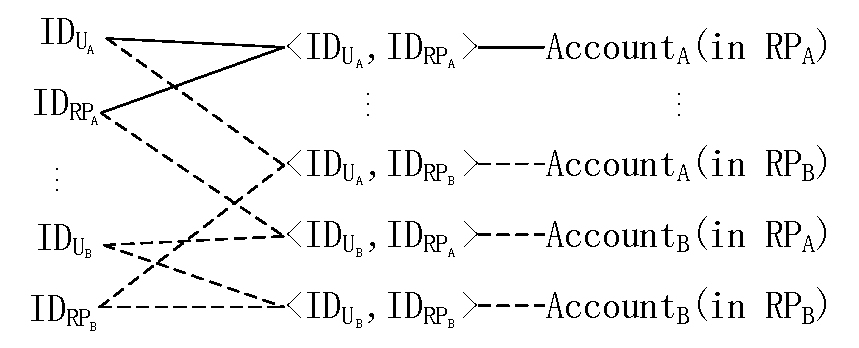
\includegraphics[width=\linewidth]{fig/link1.pdf}
  \caption{Traditional SSO.}
  \label{fig:TraditionalSSO}
\end{figure}
\begin{figure}
  \centering
  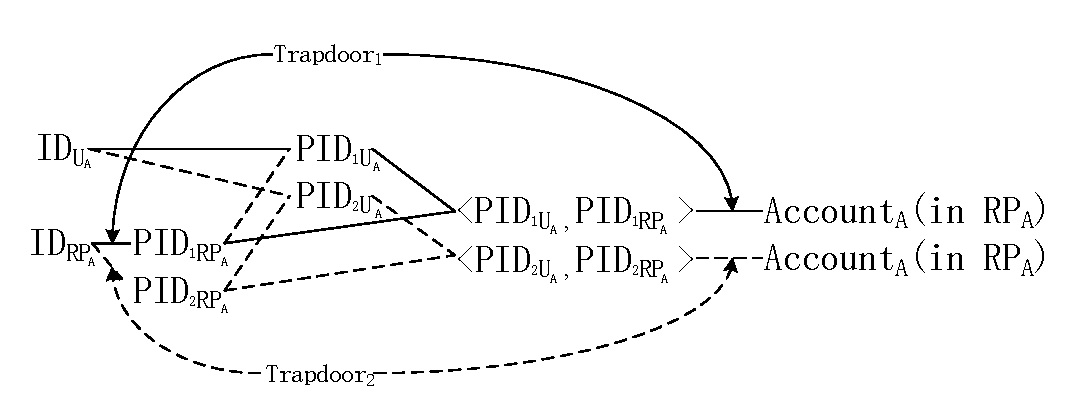
\includegraphics[width=\linewidth]{fig/link2.pdf}
  \caption{Our scheme.}
  \label{fig:Ourscheme}
\end{figure}
\begin{figure}
  \centering
  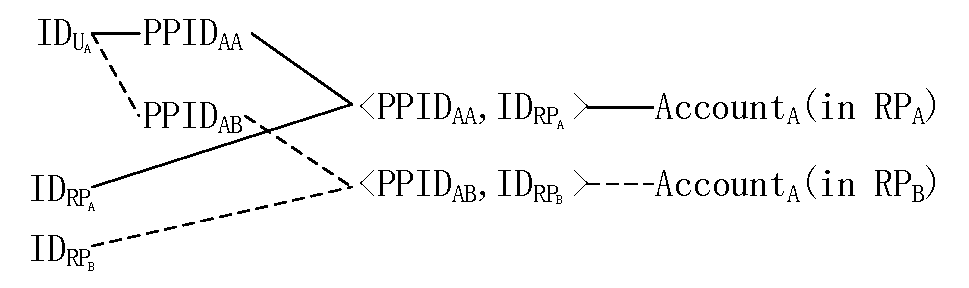
\includegraphics[width=\linewidth]{fig/link4.pdf}
  \caption{PPID.}
  \label{fig:PPID}
\end{figure}
\begin{figure}
  \centering
  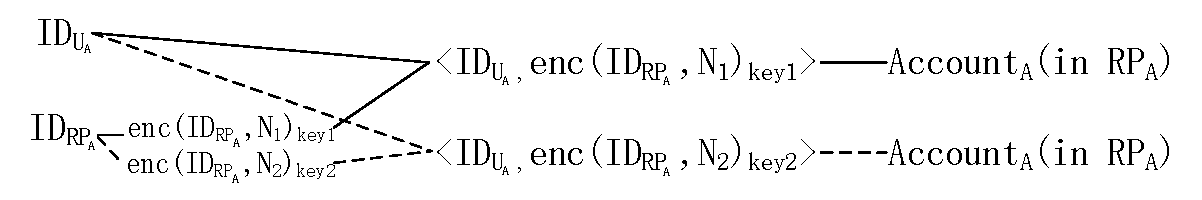
\includegraphics[width=\linewidth]{fig/link3.pdf}
  \caption{SPRESSO.}
  \label{fig:SPRESSO}
\end{figure}


%In BrowserID and SPRESSO, collusive RPs could link a user's multiple logins from the common user identifier.
%In this paper, we present UPRESSO, an Unlinkable Privacy-REspecting Single Sign-On system,
%UPRESSO, privacy-\(RE\)specting single sign-On system a\(C\)hieving un\(L\)inkable \(USE\)rs' traces
%as a comprehensive solution to tackle the privacy problems in SSO. We propose novel identifier generation schemes to dynamically generate  privacy-preserving user and RP identifiers, denoted as $PUID$ and $PRPID$, to construct identity proofs for SSO, which satisfy three properties: (1) when a same or differnt user(s) log in to a same RP, random $PRPID$s are generated in different logins so that a curious IdP cannot infer the real identity of the RP or link multiple logins at that RP; (2) when a same user logs in to a same or different RPs, random $PUID$s are generated so that
%neither a curious IdP nor
%collusive RPs cannot link the logins of that user; (3) when a same user logs in to a same RP, the RP can derive a unique user identifier from different PUIDs with a trapdoor so that it can provide a continuous service to the user during different logins.

%from both the IdP and RPs, named {UPRESSO}. To achieve this, we rely on the user to achieve the trusted transmit and correctness check of identity proof (same as in BrowserID~\cite{persona}), and propose two algorithms to achieve:



Unlike previous approaches that require non-trivial re-design of the existing SSO systems, UPRESSO can be implemented over a widely used OIDC system with small modifications with the support of its dynamic registration function~\cite{DynamicRegistration}.

%Reluse only requires the following modification on  OIDC implementations: (1) an additional web service at the IdP for providing a  set of public parameters; (2) the support for generating  the new RP identifier (at the user and RP), PPID (at the IdP) and user's account (at RP). The prototype demonstrates  that UPRESSO is incompatible with existing OIDC implementations.








%第六段
%我们的贡献
%提出协议
%考虑能否根据模型进行分析
%实现原型系统
The main contributions of UPRESSO are as follows:
\begin{itemize}
\item We systematically analyze the privacy issues in SSO systems and propose a comprehensive protection solution to hide users' traces from both curious IdPs and collusive RPs, for the first time. We also provide a systematic analysis to show that UPRESSO achieves the same level of security as existing SSO systems.
%deals with all the privacy issues introduced by SSO comprehensively. It has the ability to prevent IdP from tracking users' login trace, as well as multiple RPs are unable to link the users either.
%pratical extension for OIDC, which inherits the systematically and thoroughly analyzed  security and privacy mechanisms of OIDC, and achieves the full privacy for users by hiding the accessed RPs from IdP.
\item We develop a prototype of UPRESSO that is compatible with OIDC and demonstrate its effectiveness and efficiency with experiment evaluations.
\end{itemize}



%第七段
%文章结构
The rest of this paper is organized as follows. We introduce the background in Sections~\ref{sec:background}, and the challenges with solutions briefly~\ref{sec:challenge}. Section~\ref{sec:related} and Section~\ref{sec:UPRESSO} describe the threat model and the design of UPRESSO. A systematical analysis is presented in Section~\ref{sec:analysis}. We provide the implementation specifics and evaluation in Section~\ref{sec:implementation}, then introduce the related works in Section~\ref{sec:related}, and draw the conclusion finally.
% and Section~\ref{sec:evaluation}

